

%
%  $Description: Author guidelines and sample document in LaTeX 2.09$ 
%
%  $Author: ienne $
%  $Date: 1995/09/15 15:20:59 $
%  $Revision: 1.4 $
%

\documentclass[times, 10pt,twocolumn]{article} 
\usepackage{article}
 \usepackage[utf8]{inputenc}
\usepackage{graphicx}

%\documentstyle[times,art10,twocolumn,latex8]{article}

%------------------------------------------------------------------------- 
% take the % away on next line to produce the final camera-ready version 
\pagestyle{empty}

%------------------------------------------------------------------------- 
\begin{document}

\title{Document Classification}

\author{CPD\\
Computação Paralela e Distribuida\\
Serial+OpenMP - 2012-13\\
Tue 11h\\
 Grupo1
% For a paper whose authors are all at the same institution, 
% omit the following lines up until the closing ``}''.
% Additional authors and addresses can be added with ``\and'', 
% just like the second author.
}
	   
\maketitle
\thispagestyle{empty}

%------------------------------------------------------------------------- 
\Section{Introducão}

O objectivo deste projecto é dado um conjunto de \emph{D} documentos, cada documento classificado de acordo com \emph{S} temas e com um número \emph{C} de gabinetes, atribuir os documentos aos gabinetes baseando-se na relevância dos temas.

%-------------------------------------------------------------------------
\Section{Descrição do algoritmo e abordagem utilizada para paralelização}

Seguindo a metodologia de Foster decidimos  particionar os dados do problema pelos vários processos, isto é, dividirmos o total de documentos pelos processos, esta partição é possível pois as operações de cálculo de distâncias e de mudança de gabinete do documento podem ser realizadas independentes dos outros documentos.

O cálculo da soma dos temas de um gabinete e do total de documentos pertencente a esse gabinete também pode ser realizada independentemente dos outros documentos.

No carregamento do ficheiro para memória, os vários documentos são lidos pelo processo principal, e este envia os documentos lidos para os processos secundários.

Para o cálculo das distâncias dos documentos a cada gabinete é necessário cada processo saber as médias dos temas de todos os gabinetes, para este efeito os processo comunicam após cada cálculo da soma dos temas dos gabinetes dos seus documentos de modo a adicionar estas somas parciais e cada processo poder obter o valor de cada gabinete. Esta comunicação é global e sincronizada entre todos os processos.

Vamos então aglomerar o tarefa de cálculo de distâncias e mudança de gabinete e a tarefa de cálculo de somas de temas parciais dos gabinetes pois o cálculo anterior precisa de saber o gabinete a que cada documento pertence, esta algomeração deve-see ao facto que separar estas duas operações por processos diferentes iria levar à comunicação da posição de cada documento de um processo para o outro.

Quanto ao mapeamento do trabalho a realizar os documentos são separados em partes iguais pelos vários processos, excepto numa situação em que o número de documentos não é perfeitamente divisível pelo número de processos neste caso damos o pedaço mais pequeno ao processo principal para este se encontrar mais disponível para outras operações caso necessário.

No algoritmo descrito na Figure 1,  começamos por carregar o ficheiro em memória colocando os totais de documentos, temas e gabinetes em variáveis globais estas variáveis são enviadas no momento para os outros processos e usando dois vectores de doubles declarados \emph{static volatile}, um representa os documentos carregados e outro o estado dos gabinetes.

A distribuição dos documentos é feita pelo processo principal à media que este carrega o ficheiro em memória enviando os documentos a serem processados por cada processo, depois de carregar o ficheiro e construir as estruturas necessárias começamos com o algoritmo principal:

\begin{figure}
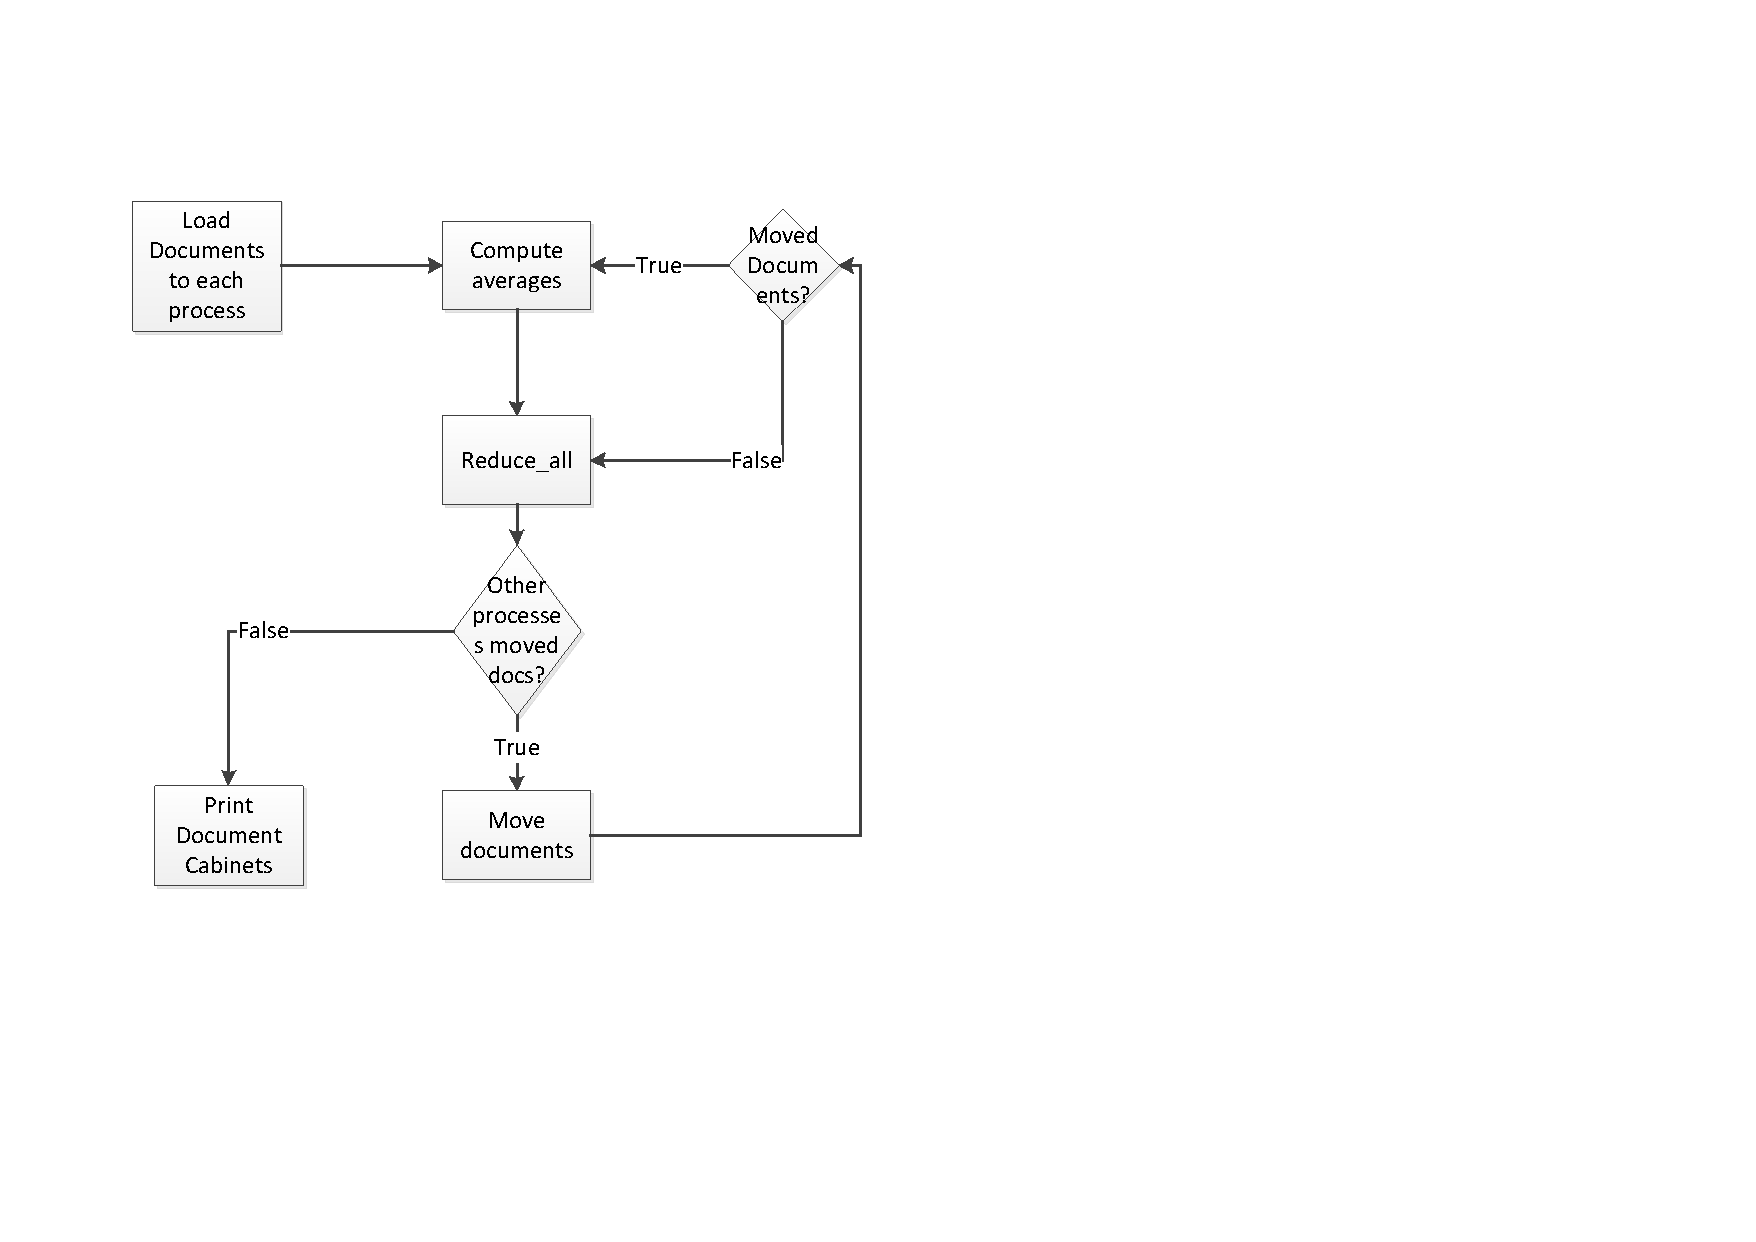
\includegraphics[width=\columnwidth]{Algoritmo.pdf}
\caption{Algoritmo usado}
\end{figure}

\begin{enumerate}
\item Calcular para cada gabinete a soma de cada tema baseado nas classificações dos temas dos documentos atribuidos ao processo, assim como o numero de documentos em cada gabinete
\item Todos os processos somam as suas somas de temas dos gabinetes e o numero de documentos contados e calculam a média de cada gabinete
\item Calcular as distâncias entre cada documento atribuído ao processo e todos os gabinetes e mover o documento para o gabinete com a menor distância;
\item Se algum documento foi mudado de gabinete ir para o passo 1, se não ir para o passo 2
\item Todos os processos comunicam para verificar se alguém moveu documentos, se ninguém moveu enviam as posições dos documentos para o processo principal e este imprime os resultados
\end{enumerate}

%No passo 1, em cada gabinete colocamos os valores dos temas a 0 e depois para cada documento verificamos se pertence ao gabinete e se pertencer adicionamos o valor dos seu temas aos valores do gabinet, depois disto para cada gabinete dividimos os valores dos seus temas pelo número de documentos atribuidos a esse gabinete.

%No passo 2, para cada documento calculamos a sua distância a cada gabinete calculando uma normal de um vector que tem como coordenadas os valores dos temas do documentos e do gabinete, e alteramos o gabinete a que o documento pertence se encontrar uma distancia mais curta.

%Após termos terminado a versão de série, começamos por identificar as tarefas primitivas de entre as várias funções criadas.
%Depois efectuou-se a alteração do código de forma a permitir aplicar um maior paralelismo ao código e garantir a independência do acesso à memória no acesso às estruturas de dados.
%Com a análise inicial passou-se a uma análise mais aprofundada apoiada nos resultados obtidos.


%-------------------------------------------------------------------------
\Section{Decomposição, Sincronização e Balanceamento de Carga}

\SubSection{Loading Data}

Na leitura do ficheiro e carregamento dos dados o processo principal vai lendo o ficheiro e primeiro realiza um Broadcast para distribuir um vector de inteiros que incluí os totais lidos das primeiras linhas.

E depois divide os documentos igualmente pelos processos, quando o processo principal tiver lido os documentos sobre os quais um processo secundário vai trabalhar, o processo principal realiza um Send com vector parcial com os documentos, e continua a ler o ficheiro após o envio, quando acabar de distribuir os pedaços pelos vários processos secundários, o processo principal fica com o ultimo pedaço do vector dos documentos.

A decisão de enviar os pedaços de documentos à medida que são lidos permite que os processos que recebem logo os seus documentos começarem a trabalhar enquanto o processo principal ainda está a carregar o ficheiro.

Quanto ao processo principal ficar com o ultimo pedaço foi decidido de modo ao processo principal ter em certos casos menos documentos que os processos secundários e assim se encontrar mais disponível para operações extraordinárias, estas no entanto não se verificam pois as nossas zonas de comunicação entre os processos são poucas e simples.

%Na paralelização dos dados existem duas tarefas primitivas que se podem identificar:
%- leitura dos dados do ficheiro
%- conversão de strings para valores numéricos que podem ser int (id do documento) ou doubles (rate do subject)
%
%Nesta parte verificou-se que havia problemas com a ordem de leitura tendo em conta o formato do ficheiro de entrada que não permite que haja muita paralelização. Esta observação surge por não ser vantajoso manter mais do que um file descriptor activo para efectuar leitura do mesmo ficheiro em zonas diferentes, pois o overhead acabava por cair sobre o próprio IO que é muito penalizante para o funcionamento em shared memory.
%Desta forma, verificou-se que, estando a correr ao nível da mesma máquina, não se tem vantagens em paralelizar as leituras de IO. No entanto consegue-se ganhar alguma vantagem na paralelização das escritas para a memória durante as leituras dos dados, na medida que a criação dos documents não tem a restrição de seguir a ordem de leitura, tendo em conta a estrutura de dados adoptada. No caso dos subjects consegue-se também algum paralelismo na medida que durante a leitura do ficheiro é possível estar a realizar as conversões a partir do buffer em paralelo.
%Analisou-se também a influência de se ter schedule aplicado no for interior de leitura dos vários subjects por linha, fazendo variar o valor de chunks associado a dynamic e guided. Neste caso verificou-se que guided se tornava mais eficiente, na medida que a master thread tem sempre bastante trabalho com a leitura do ficheiro e depois as escritas na memória eram efectuadas em paralelo. No entanto, o peso que tinha o controlo dos vários fork e joins constantes num ciclo muito interior, demonstrou não trazer vantagem, mesmo com o balanceamento de carga e manipulação dos valores de chunk.
%De acordo com os resultados apresentados e tendo em conta as restrições de ordem não se conseguiu paralelizar mais esta parte do código.

\SubSection{Cálculo de Médias}
Cada processo tem aproximadamente documentos/processos documentos guardados, para calcular as médias dos gabientes cada processo soma os vários temas de cada documento pertencente a um gabinete e conta o número de documentos que cada gabinete tem.

Estas somas são guardadas num vector de doubles que, por exemplo, se tivessemos 3 gabinetes com 2 temas cada teria a estrutura na Figure 2. 

Neste vector de doubles são guardados os temas de cada gabinete separados pelo contador dos documentos que cada gabinete tem atribuídos a ele no final do vector tem uma flag que é usada para saber se o processo moveu documentos de gabinetes no passo anterior, na 1ª execução do compute averages esta flag é colocada a 1 e alterada mais tarde pela função que move os documentos entre gabinetes.

\begin{figure}
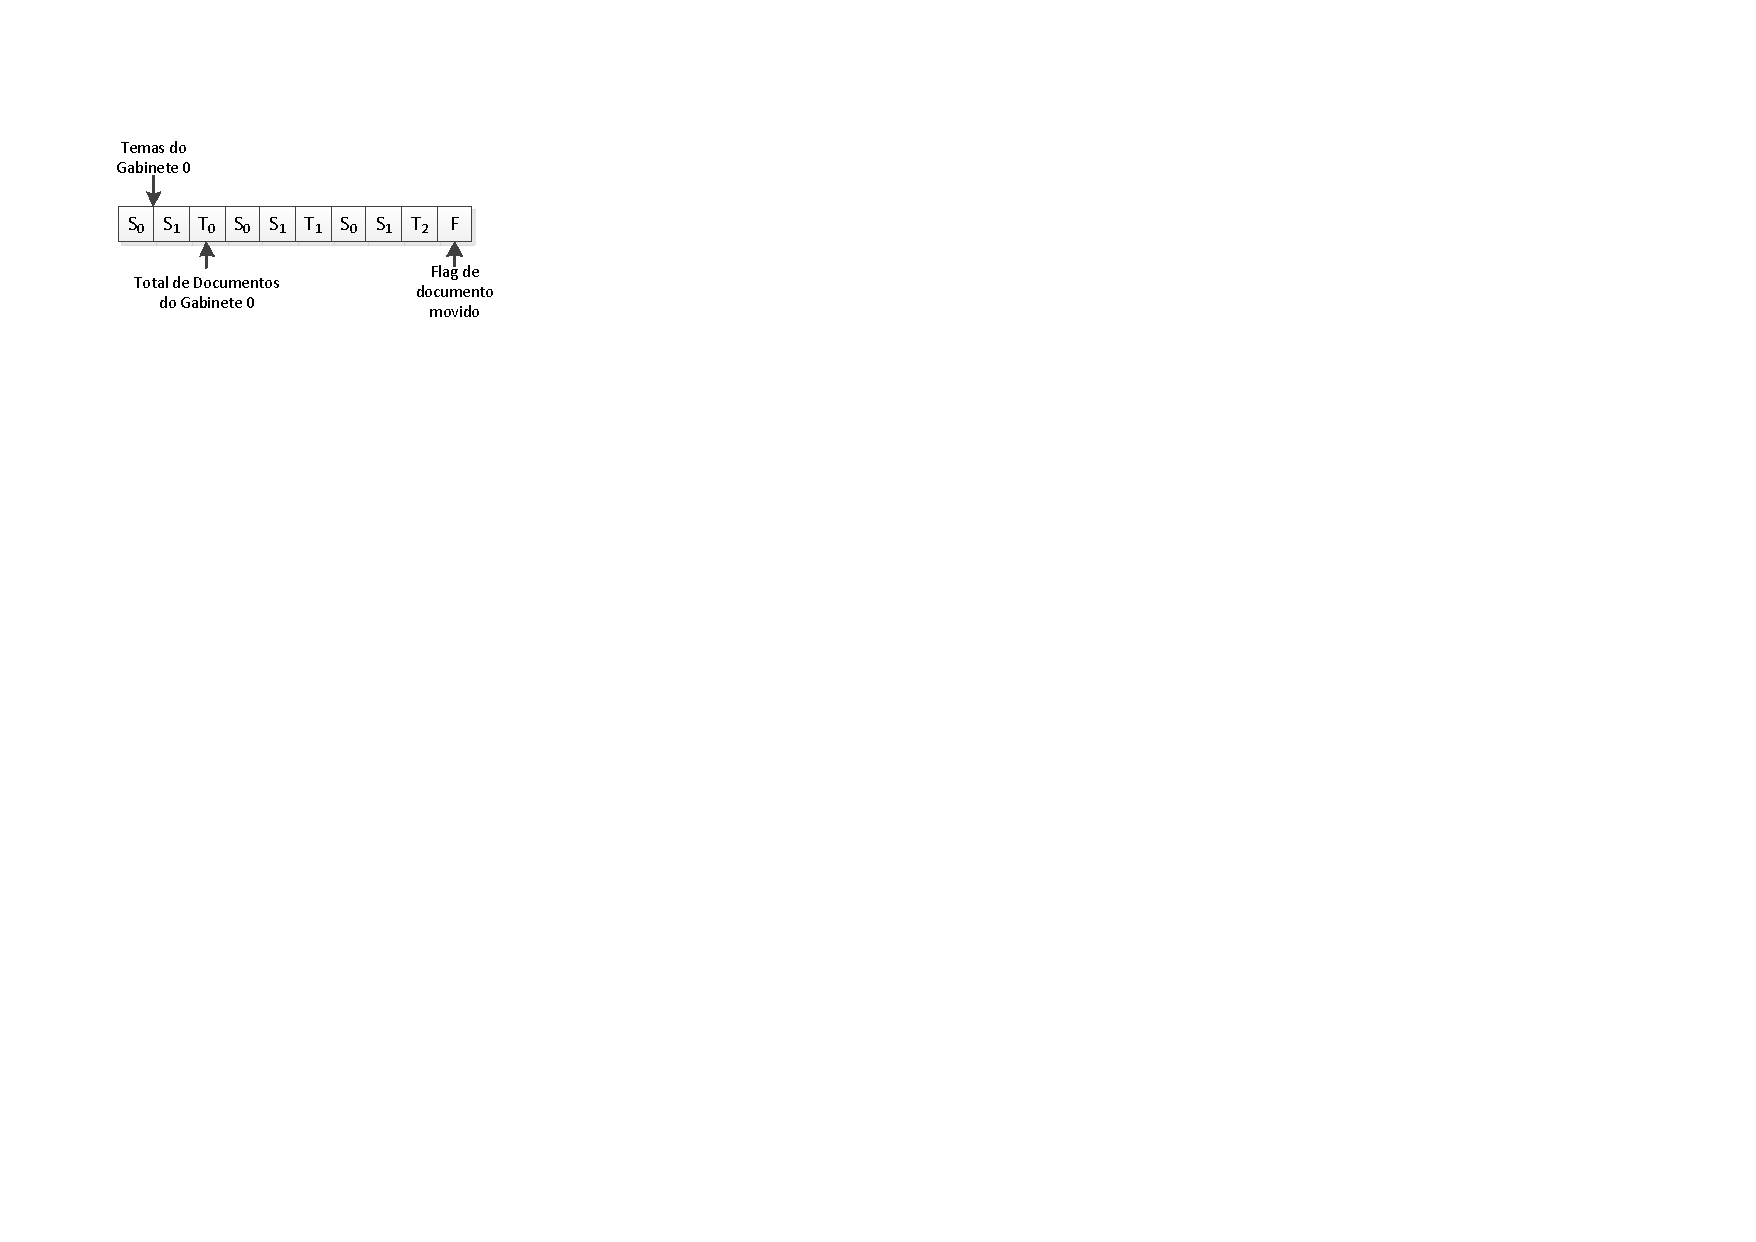
\includegraphics[width=\columnwidth]{VectorGabinete.pdf}
\caption{Estrutura do Vector de Gabinetes}
\end{figure}

Depois destas somas estarem calculadas para todos os gabinetes, é feito um AllReduce do vector dos gabinetes de cada processo de modo a todos os processos terem os totais globais, a estrutura do vector permite que isto seja feito apenas com um ALLReduce sem a necessidade de realizar operações separadas para as diferentes somas, cada processo então realiza a divisão final entre os temas e o número de documentos para calcularem a média dos gabinetes.

%Calculamos as médias atribuindo os gabinetes às threads disponiveis, isto levanta problemas de \emph {load balancing} quando, temos menos gabinetes que threads disponiveis e quando nos passos do algoritmo principal cada gabinete pode ter um total de documentos atribuidos diferentes o que leva a divisão de trabalho diferente entre threads.
%
%De modo a tentar resolver este problema de gestão de trabalho tentámos alterar a maneira como calculamos as médias.
%
%Alterando a ordem dos fors em cascata que usamos, tentamos dividir os documentos em vez dos gabinetes pelas threads mas isto trouxe problemas de sincronização e atrasos na execução devido a termos várias threads a tentarem alterar o mesmo valor do gabinete.
%
%Tentámos a paralelização dos for’s interiores da solução original mas esta solução trouxe problemas na quantidade de overhead adicional devido à constante criação de threads.
%
%Tentamos também efectuar a paralelização mantendo o ciclo for exterior e adicionando um ciclo for interior que se traduz numa situação de neasted parallelism. Porque havia necessidade de sincronização dos dados em termos de acessos a memória pela necessidade de todos os processos associados ao ciclo que percorre todos os documentos, verificou-se que o overhead de comunicação e de controlo se tornava mais pesado do que a vantagem que se tirava do paralelismo. 
%Experimentou-se mesmo correr o parallel for exterior com shedulle dynamic e gided com chunks de 1, 2 e 4 em que se conseguia apenas pequenas optimizações na execução para testes maiores e com uma cobertura de paralelização do código de mais de 90%, mas agravava os problemas de concorrência pela memória, o que tornava o tempo de execução mais lento.
%Para analisar a revelância ao nível de comunicação e controlo experimentou-se criar tasks para a tarefa primitiva da soma dos valores em vez do for. Uma vez mais demonstrou não trazer vantagem para além de não se ter conseguido evitar os problemas de concorrência de dados que resultavam em resultados errados.
%
%No final a solução inicial foi a escolhida porque mostrou ter a melhor performance entre todas as alternativas testadas.



\SubSection{Calcular Distâncias}
Quando o vector de Gabinetes se encontrar actualizado os vários processos vão calcular as distâncias aos gabinetes de cada um dos seus documentos e movê-los se tal for o caso. De seguida o processo altera a sua Flag no vector de Gabinetes se este processo tiver movido algum documento

Se a Flag de documento movido estiver a 0 o processo não recalcula novas somas para os Gabinetes pois tem as somas guardadas da iteração anterior, e estas matêm-se iguais pois nenhum dos seus documentos mudou de posição, o processo então salta para o passo de AllReduce.

No passo a seguir ao cálculo das médias é que é testada a condição de paragem do algoritmo, após o AllReduce se um ou mais processos tiverem movido documentos, a Flag irá se encontrar maior que zero em todos os processos então estes sabem que o algoritmo ainda não parou e devem continuar.

%Ao calcular as distâncias separamos os documentos entre as threads disponiveis usando um simples \emph{pragma omp for} e colocando as variaveis auxiliares na lista \emph{private} esta provou ser a solução mais simples e rápida.
%
%Esta implementação garante uma distribuição de trabalho entre as threads pois todos os documentos têm a mesma quantidade de trabalho, e como os documentos são independentes entre eles não existe zona crítica.
%
%Uma alteração adicional que nos ajudou a obter melhores tempos foi o uso de uma variavel auxiliar na lista private, esta variável era do tipo Cabinet* e foi declarada static volatile, pensamos que isto ajudou na execução diminuindo o número de invalidações de cache quando as threads queriam aceder ao vector principar de gabinetes.
%
%Conseguiu-se também aumentar o paralelismo ao colocar o document a analisar como variável local em vez de se estar a passar o vector de documents. Desta forma document era recebido por cada tarefa como firstprivate e permitiu o acesso concorrente às várias posições do vector, que são preenchidas independentemente.
%
%Com estas várias modificações do código em relação à versão de série conseguiu-se uma cobertura de paralelismo do código de mais de 90% e sem problemas de incoerência de dados. Esta foi a tarefa primitiva onde se consegiu atingir o maior paralelismo e por sua vez a maior performance.


%-------------------------------------------------------------------------
\Section{Resultados Obtidos}

Devido à problemas inprevistos no desenvolvimento da nossa solução e devido à enorme afluência de processos ao nível do cluster não tivemos tempo suficiente para testar e analisar a fundo a performance da nossa solução.

Esta solução que entregamos junto com este relatório foi capaz de correr a maiorias dos nossos testes realizados.

Também entregamos uma versão do docs-omp-mpi.c que no momento desta entrega se encontrava a funcionar correctamente em todos os nossos testes, excepto eventuais problemas com as ocupações das máquinas. Esta versão funciona distribuída nas várias máquinas fornecidas com o comando availableNode e é possível usar a variável global para definir o número de threads a correr em cada processo.


%Todos os tempos de execução foram medidos usando máquinas dos laboratórios da RNL, os tempos de execução para cada teste são as médias de 6 execuções.
%Para ajudar com avaliação criá-mos 2 testes novos:
%\begin{itemize}
%\item ex100m-100d.in um teste com os cem mil primeiros documentos do teste ex1M-100d.in e mantendo o mesmo número de Gabinetes e Sujeitos
%\item ex10m-100d.in um teste com os dez mil primeiros documentos do teste ex1M-100d.in e mantendo o mesmo número de Gabinetes e Sujeitos
%\end{itemize}
%
%Primeiro mostramos um gráfico com uma escala logaritmica dos tempos de execução obtidos:
%
%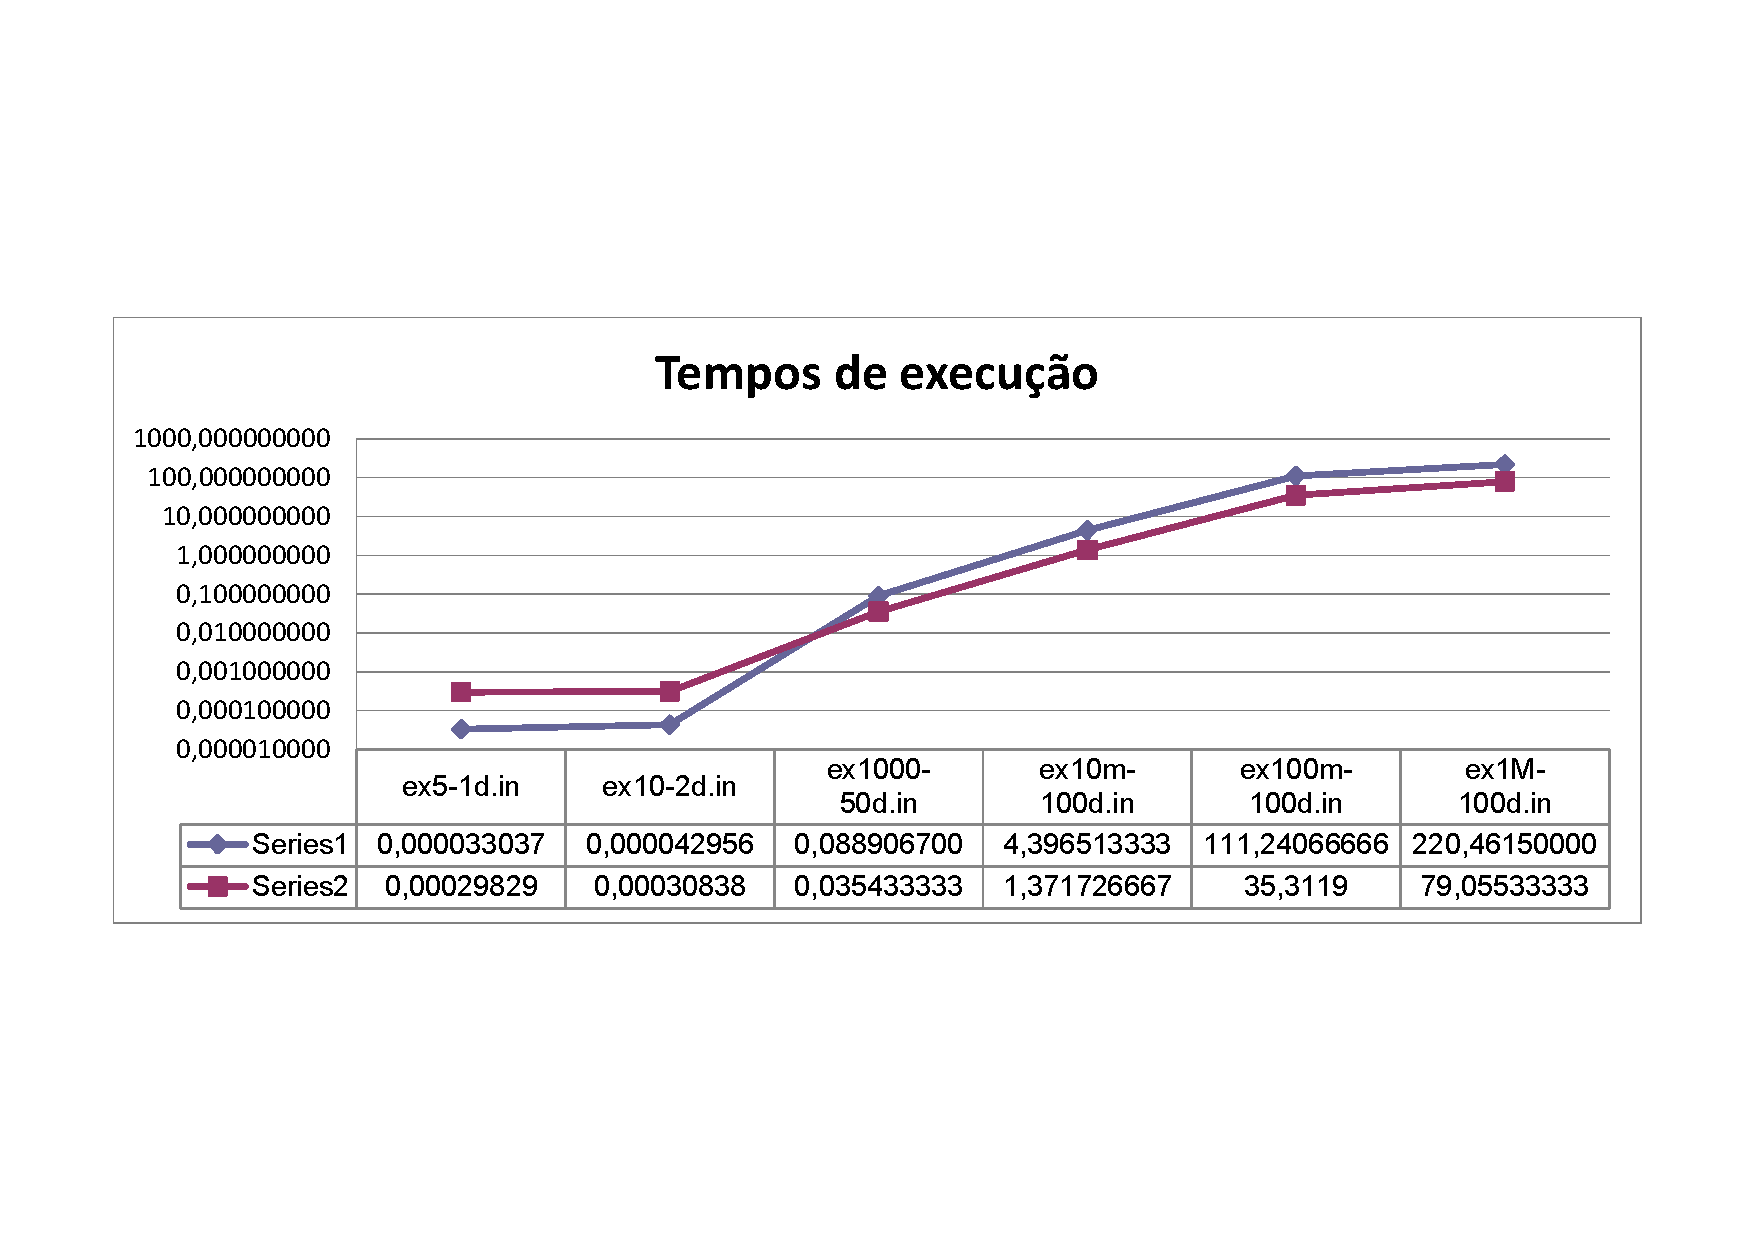
\includegraphics[width=\textwidth]{tempos.pdf}
%
%Por esta tabela podemos ver que os testes iniciais têm na verdade um atraso em relação aos de série devido ao overhead da criação de threads, mas após 3 teste começamos a observar melhoramentos nos tempos de execução.
%
%No gráfico seguinte mostramos o Speedup calculado usando os tempos acima obtidos:
%
%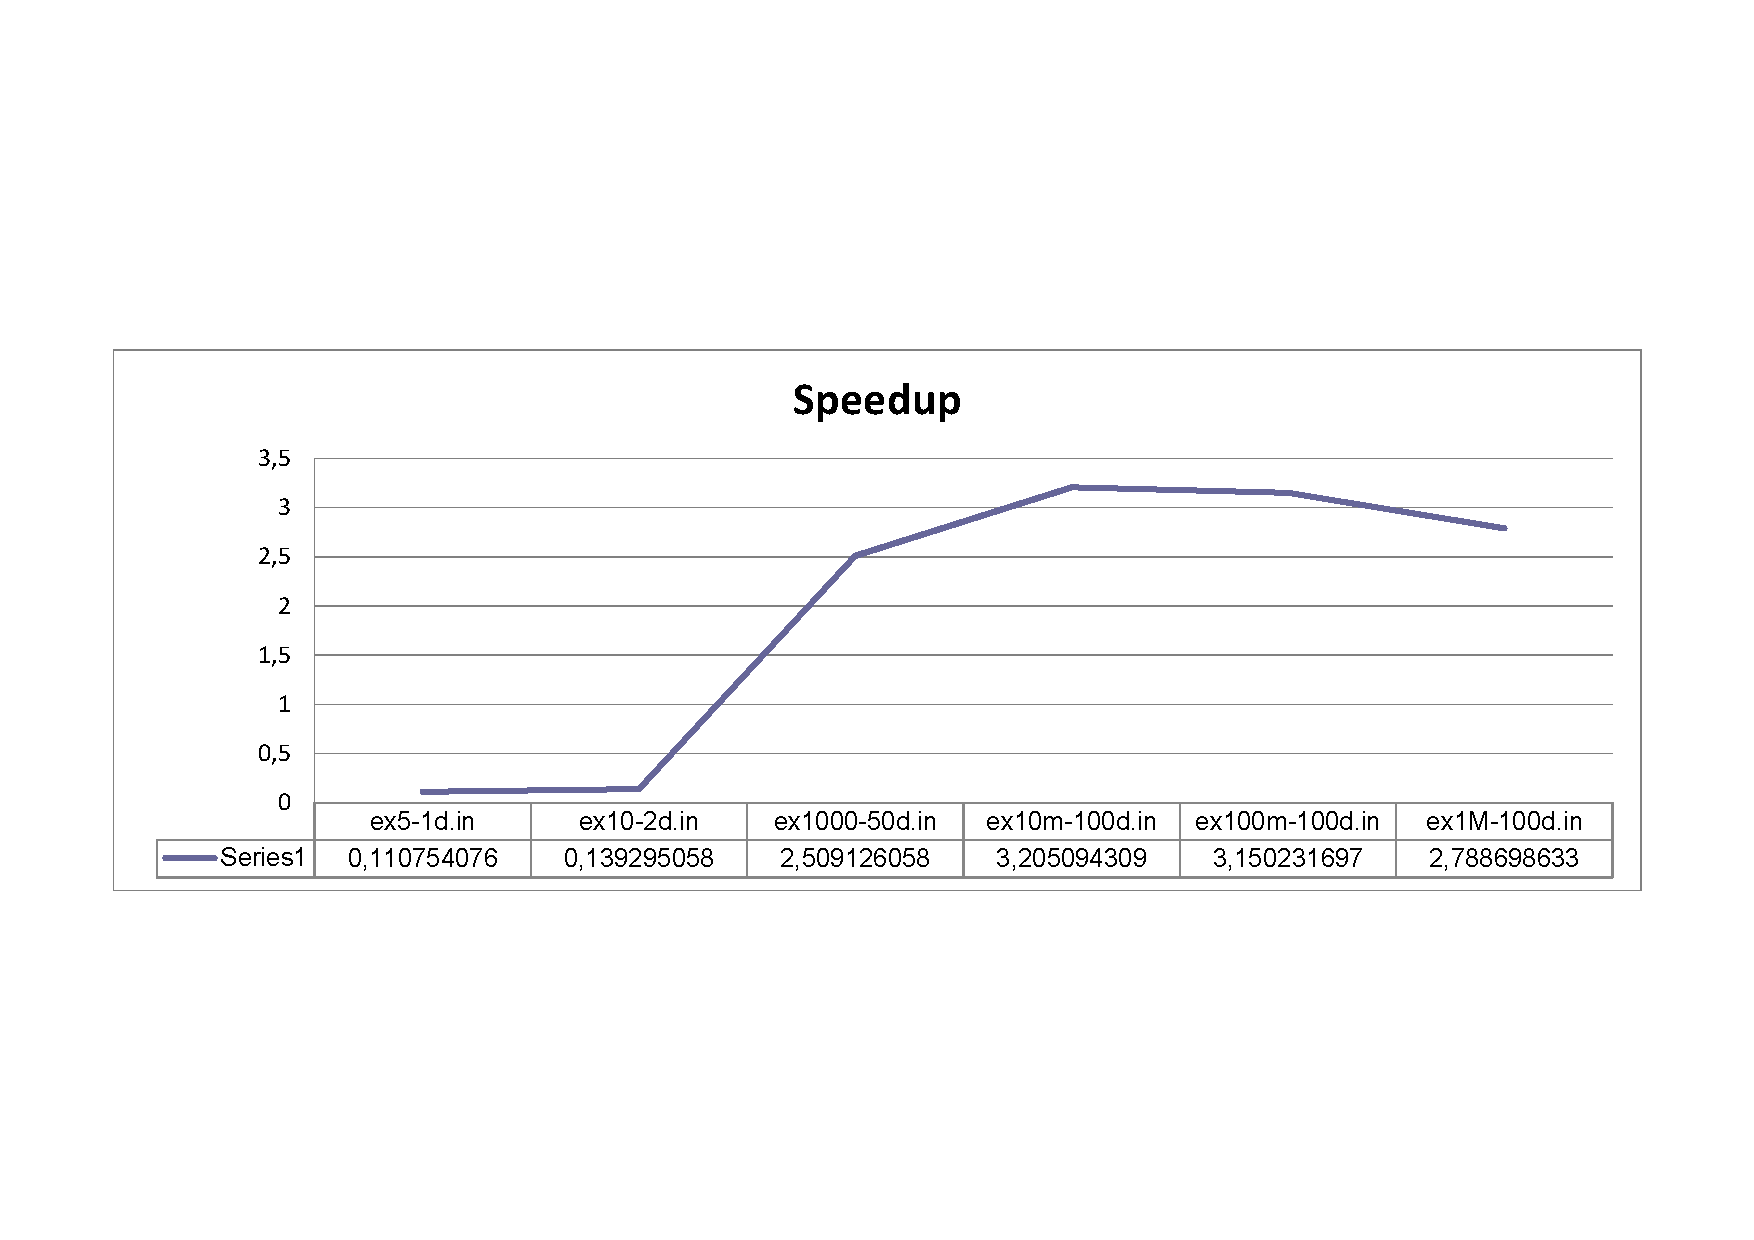
\includegraphics[width=\textwidth]{speedup.pdf}
%
%Excluindo os 2 teste inicais obtemos speedups entre os 2,4 e 3.5 o que demonstra uma considerável eficiência na paralelização do algoritmo.

%-------------------------------------------------------------------------


%------------------------------------------------------------------------- 

\end{document}

